%
% The first command in your LaTeX source must be the \documentclass command.
\documentclass[sigchi-a]{acmart}
\usepackage{anyfontsize}
%
% defining the \BibTeX command - from Oren Patashnik's original BibTeX documentation.
\def\BibTeX{{\rm B\kern-.05em{\sc i\kern-.025em b}\kern-.08emT\kern-.1667em\lower.7ex\hbox{E}\kern-.125emX}}
    
% Rights management information. 
% This information is sent to you when you complete the rights form.
% These commands have SAMPLE values in them; it is your responsibility as an author to replace
% the commands and values with those provided to you when you complete the rights form.
%
% These commands are for a PROCEEDINGS abstract or paper.
%\acmConference[CHI'19]{ACM CHI Conference on Human Factors in Computing Systems}{May 2019}{Glasgow, Scotland, UK}
%\acmYear{2019}
%\setcopyright{acmlicensed}

%\copyrightyear{2018}
%\acmYear{2018}
%\setcopyright{acmlicensed}
%\acmConference[Woodstock '18]{Woodstock '18: ACM Symposium on Neural Gaze Detection}{June 03--05, %2018}{Woodstock, NY}
%\acmBooktitle{Woodstock '18: ACM Symposium on Neural Gaze Detection, June 03--05, 2018, Woodstock, %NY}
%\acmPrice{15.00}
%\acmDOI{10.1145/1122445.1122456}
%\acmISBN{978-1-4503-9999-9/18/06}

%
% These commands are for a JOURNAL article.
%\setcopyright{acmcopyright}
%\acmJournal{TOG}
%\acmYear{2018}\acmVolume{37}\acmNumber{4}\acmArticle{111}\acmMonth{8}
%\acmDOI{10.1145/1122445.1122456}

%
% Submission ID. 
% Use this when submitting an article to a sponsored event. You'll receive a unique submission ID from the organizers
% of the event, and this ID should be used as the parameter to this command.
%\acmSubmissionID{123-A56-BU3}

%
% The majority of ACM publications use numbered citations and references. If you are preparing content for an event
% sponsored by ACM SIGGRAPH, you must use the "author year" style of citations and references. Uncommenting
% the next command will enable that style.
%\citestyle{acmauthoryear}

%
% end of the preamble, start of the body of the document source.

%WISH Poster
\copyrightyear{2019}
\acmYear{2019}
\setcopyright{rightsretained}
\acmConference[WISH'19 Poster, CHI 2019 Conference on Human Factors in Computing Systems\\May 4--9, 2019, Glasgow, Scotland UK]{}{}{}
\fancyhead{}

\begin{document}

%
% The "title" command has an optional parameter, allowing the author to define a "short title" to be used in page headers.
\title{A novel hand-held interface supporting the self-management of type 1 diabetes}

%
% The "author" command and its associated commands are used to define the authors and their affiliations.
% Of note is the shared affiliation of the first two authors, and the "authornote" and "authornotemark" commands
% used to denote shared contribution to the research.
%\author{Robert Spence, Chukwuma Uduku, Kezhi Li, Pantelis Georgiou}
%\authornote{R. Spence, K. Li and P. Georgiou are with Depertment of Electrical and Electronic Engineering, Imperial College London. C. Uduku is with Department of Medicine, Imperial College London. K. Li is the corresponding author. The work was supported by EPSRC EP/P00993X/1.}
%\email{{r.spence,chukwuma.uduku04,kezhi.li,pantelis}@imperial.ac.uk}
%\orcid{1234-5678-9012}
%\author{G.K.M. Tobin}
%\authornotemark[1]
%\email{webmaster@marysville-ohio.com}
%\affiliation{%
%  \institution{Imperial College London, United Kingdom}
%  \streetaddress{South Kensington}
%  \city{London}
%  \state{United Kingdom}
%  \postcode{SW7 2AZ}
%}


\author{Robert Spence}
\affiliation{%
  \institution{Dept. of Electrical and Electronic Engineering}
%  \streetaddress{South Kensington}
%  \city{London}
  \country{Imperial College London, United Kingdom}
}
\email{r.spence@imperial.ac.uk}

\author{Chukwuma Uduku}
\affiliation{%
  \institution{Dept. of Medicine}
%  \streetaddress{South Kensington}
%  \city{London}
  \country{Imperial College London, United Kingdom}
}
\email{chukwuma.uduku04@imperial.ac.uk}

\author{Kezhi Li}
\affiliation{%
  \institution{Dept. of Electrical and Electronic Engineering }
%  \streetaddress{South Kensington}
%  \city{London}
  \country{Imperial College London, United Kingdom}
}
\email{kezhi.li@imperial.ac.uk}

\author{Pantelis Georgiou}
%\authornote{The work was supported by EPSRC EP/P00993X/1. K. Li is the corresponding author. }
\affiliation{%
  \institution{Dept. of Electrical and Electronic Engineering}
%  \streetaddress{South Kensington}
%  \city{London}
  \country{Imperial College London, United Kingdom}
}
\email{pantelis@imperial.ac.uk}

%\author{Valerie B\'eranger}
%\affiliation{%
%  \institution{Inria Paris-Rocquencourt}
%  \city{Rocquencourt}
%  \country{France}
%}



%
% The abstract is a short summary of the work to be presented in the article.
\begin{abstract}
%For pressing economic and social reasons a hand-held interactive interface supporting the self-management of a chronic condition has much to offer. We describe the design of such an interface specifically for people with Type-1 diabetes, but it is potentially generalizable to other chronic conditions.  A major consideration in the design of the interface is the support that visible context can provide.  Within this consideration a diary permits both qualitative and quantitative viewing of temporal data, and complex relations between many clinical and user-selected variables can be explored manually and dynamically.

For pressing health, economic and social reasons a hand-held interactive interface supporting the self- management of a chronic condition has much to offer.

We describe the design of an interface specifically for people with Type-1 diabetes, but it is potentially generalizable to other chronic conditions.  Three sets of constraints influenced the design. One derives from clinical considerations. Another recognizes the preferences of users, expressed as inherent interests or reactions to successive interface designs. A third constraint arises from the small size of the hand-held device. 

Considerations of all three constraints, as well as accepted guidelines concerning design for human-system interaction, led to the novel interface described in this paper. The principal features include: a very `flat' data space; the extensive use of visible context; techniques to ease menu selection by the visually impaired; an interactive diary displaying both qualitative and quantitative aspects of data; and the dynamic manual exploration of interrelationships.  
\end{abstract}

%
% The code below is generated by the tool at http://dl.acm.org/ccs.cfm.
% Please copy and paste the code instead of the example below.

%
% Keywords. The author(s) should pick words that accurately describe the work being
% presented. Separate the keywords with commas.
%\keywords{datasets, neural networks, gaze detection, text tagging}

%\begin{CCSXML}
%<ccs2012>
%<concept>
%<concept_id>10003120.10003121.10003124</concept_id>
%<concept_desc>Human-centered computing~Interaction paradigms</concept_desc>
%<concept_significance>300</concept_significance>
%</concept>
%<concept>
%<concept_id>10003120.10003123.10010860.10010858</concept_id>
%<concept_desc>Human-centered computing~User interface design</concept_desc>
%<concept_significance>300</concept_significance>
%</concept>
%</ccs2012>
%\end{CCSXML}
%
%\ccsdesc[300]{Human-centered computing~Interaction paradigms}
%\ccsdesc[300]{Human-centered computing~User interface design}

%\keywords{Mobile devices; health; interaction design}


\settopmatter{printacmref=false}
%
% A "teaser" image appears between the author and affiliation information and the body 
% of the document, and typically spans the page. 
%%\begin{teaserfigure}
%%  \includegraphics[width=\textwidth]{sampleteaser}
%%  \caption{Seattle Mariners at Spring Training, 2010.}
%%  \Description{Enjoying the baseball game from the third-base seats. Ichiro Suzuki preparing to bat.}
%%  \label{fig:teaser}
%%\end{teaserfigure}

%
% This command processes the author and affiliation and title information and builds
% the first part of the formatted document.

\maketitle

%\begin{margintable}
%  \caption{This work is supported by EPSRC.}
%\end{margintable}

%\begin{sidebar}
%\fontsize{10}{12}{\textbf{KEYWORDS}}\\
%\normalsize{Mobile devices; health; interaction design}
%\end{sidebar}

\begin{sidebar}
%use vspace to place your sidebar at the right position
%\vspace{.5cm}
\textbf{KEYWORDS}\\
Mobile devices; health; interaction design
\end{sidebar}

\linespread{0.95}

\section{Introduction}

%The prevalence of chronic disease is rising on a global scale due to advances in general healthcare. 
In light of the prevalence of chronic disease and its associated economic and social consequences, a hand-held application allowing a patient to self-manage their condition has much to offer.
Suboptimal care in this population comes with a significant socioeconomic burden arising from physical and psychosocial complications. Mobile health applications are cost-effective tools that empower users to better understand and self-manage their conditions.



Type 1 diabetes (T1DM) is a chronic condition characterized by insulin insufficiency due to the autoimmune destruction of pancreatic beta cells \cite{oviedo2017review}. Subcutaneously administered insulin replacement therapy is the mainstay of treatment, and can be delivered as multiple daily injections or via a continuous subcutaneous insulin infusion pump. Diabetes health applications have been shown to successfully improve treatment outcomes (e.g., blood glucose control), health behaviour (e.g., self-monitoring of blood glucose), patient self-confidence, and patient satisfaction \cite{Bonoto-EffOfMob2017}. However, a study \cite{Connell-23ofUsers2017} from the leading mobile engagement platform found that a quarter of users abandon apps after just one use, with poor software user experience being a major barrier in mobile health application penetration. Therefore, a primary objective when developing the health app interface described in this paper was to ensure usability across a wide demographic without compromising the following;


1.	Manual data input (e.g. meal selection and exercise intensity);
2.	Automated input of physiological parameters from wearable devices (e.g., blood glucose levels and heart rate);
3.	Presentation, to the user, of recommended treatment (e.g., insulin dosage and risk aversion strategies);
4.	Real-time visual presentation of predicted outcomes that would follow from treatment recommended by machine learning algorithms;
5.	Manual dynamic exploration of interrelations between relevant parameters (e.g., carbohydrates, predicted blood glucose and insulin recommendation).

\section{Background}

\begin{marginfigure}
\begin{minipage}[b]{0.5\linewidth}
\centering
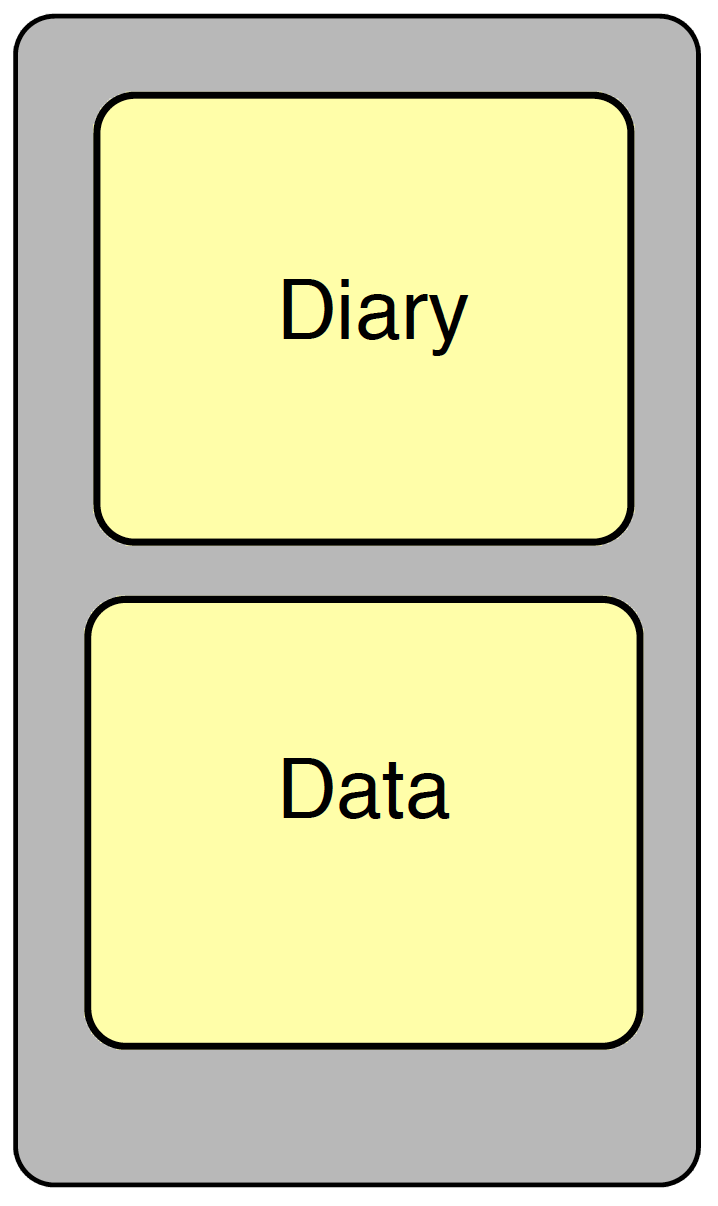
\includegraphics[height=1.5in]{fig/fig1.png}
%\caption{The allocation of display area to temporal data (top) and data input and output (lower). }
\end{minipage}% <- this is important here
\begin{minipage}[b]{0.5\linewidth}
\centering
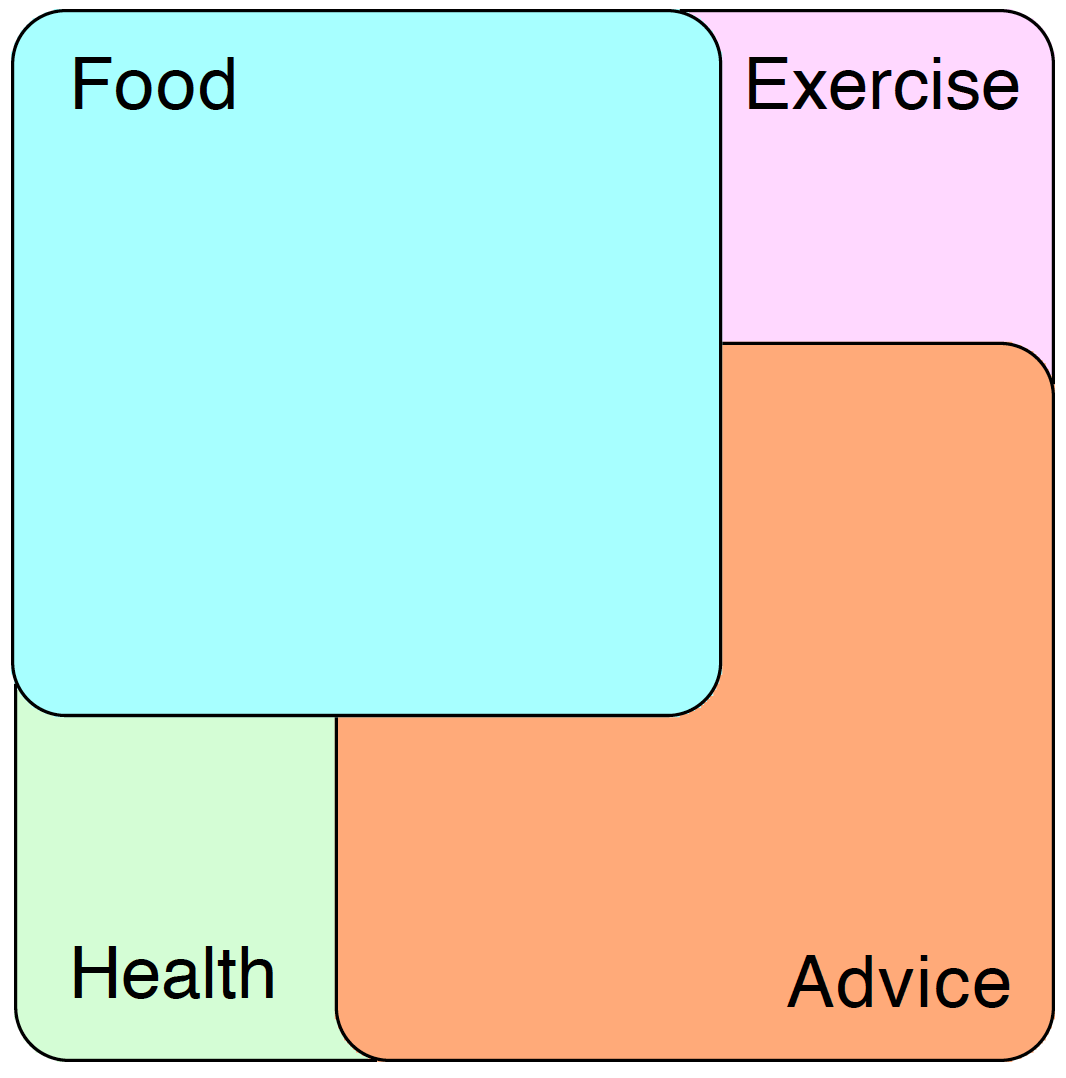
\includegraphics[height=1.5in]{fig/fig2.png}
%\caption{Layout of the four data regions occupying the lower part of the hand-held display.}
\end{minipage}
\caption{Left: The allocation of display area to temporal data (top) and data input and output (lower). Right: Layout of the four data regions occupying the lower part of the hand-held display.}
\end{marginfigure}



%Type 1 diabetes is a chronic condition requiring regular blood glucose monitoring and adjustment of insulin dosage according to activities of daily living such as eating and exercise. Continuous glucose monitoring sensors and insulin bolus (see glossary) calculators are existing technologies proven to facilitate self-management by improving glucose control and the reduction of hypoglycaemia associated with excess insulin dosage. Continuous glucose monitoring devices use a subcutaneously deployed sensor and Bluetooth technology to feed back real-time interstitial fluid glucose levels to the user's smartphone. Insulin bolus calculators are increasingly being integrated into glucose metering software, and use patient entered carbohydrate content to calculate an appropriate insulin dose corresponding to food intake. 
The majority of diabetes health apps provide treatment decision support by presenting automatic and manually entered data inputs from existing diabetes technologies in a meaningful fashion \cite{Pesl-AnAdvBolus2016}. Arsand et al \cite{Arsand-MobHeaApp2012} used various end-user-based assessments to evaluate the functionality of ten diabetes mobile health app features and outlined key components for future app development. Important features included; use of automatic data transfer, motivational and visual interface design, greater health benefit-to-effort ratio, dynamic usage, and applying context to app output.
%Herrero et al \cite{Herrero-AdvInsBolus2015} analysed how various human and environmental factors, such as exercise, stress and alcohol consumption, influence blood glucose levels and how these parameters can be incorporated in intelligent decision support systems


A review of commercially available diabetes health apps \cite{Wu-MobileApp2017} established that having a structured display was a feature that significantly improves blood glucose control. This association is likely a result of positive health behavior changes in response to well-presented health outcomes (e.g. blood glucose data). 
%A randomized cross-over study investigating glucose prediction as part of a diabetes decision support system revealed further decision modification in 20\% of cases during the experiment arm \cite{Perez-DecisionSup2018}. 
The presentation of structured glucose prediction data generated from an AI with self-learning capabilities and the ability to take account of real-time physical activity provides an opportunity to engage the user and further improve clinical outcomes \cite{Li-CRNNforGP2019}. The presence of educational and lifestyle modification features are also low risk additions that increase self-awareness and improve glucose control \cite{Wu-MobileApp2017}.
%The T1DM population comprises people from different cultural and generational backgrounds with varied ideas about, and experience with, the use of mobile health applications. 
Interface design for most diabetes decision support apps struggles to efficiently permit layered multi-source data inputs and present various outputs (e.g. blood glucose and insulin dose recommendation) without compromising ease of use, context and the number of device interactions. The app ARISES (An Adaptive, Real-time, Intelligent System to Enhance Self-care of chronic disease) described in this paper aims to overcome these hurdles by adopting evidence derived from the current literature and by including patients with varied exposure to technology within the design framework.

\begin{marginfigure}
\centering
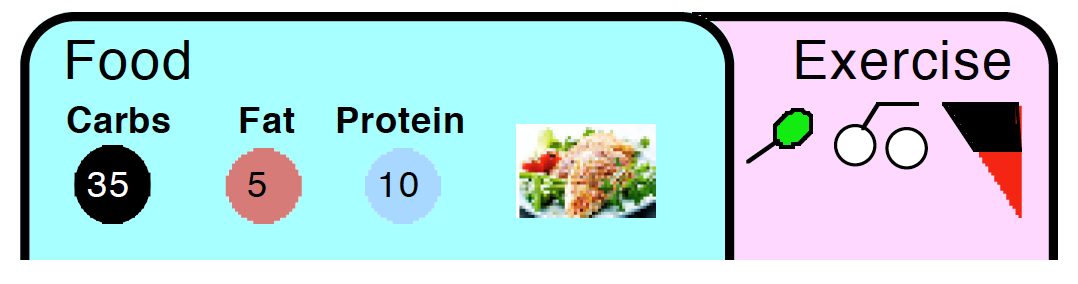
\includegraphics[height=0.7in]{fig/fig3.png}
\caption{Examples of the data concerning Food and Exercise that the patient can enter. Note that part of the Exercise area is always visible while data concerning Food is being provided by the patient.}
\end{marginfigure}

\begin{marginfigure}
\centering
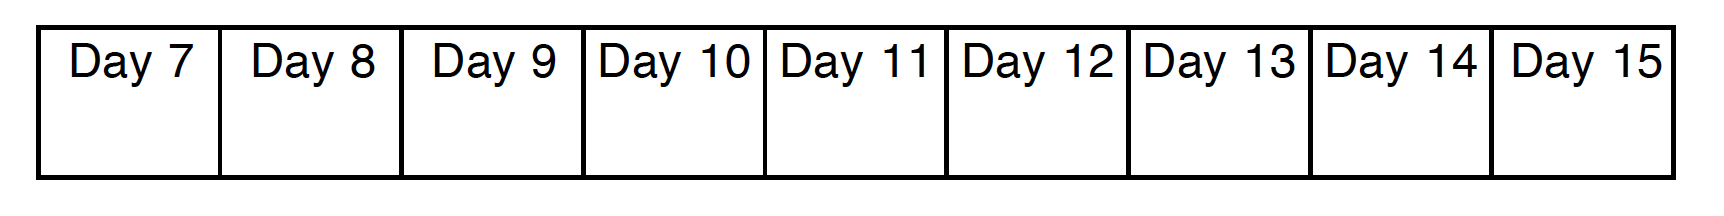
\includegraphics[height=0.37in]{fig/fig4.png}
\caption{A linear presentation of consecutive days, having a shape unsuited to a limited display area}
\end{marginfigure}

\begin{marginfigure}
\centering
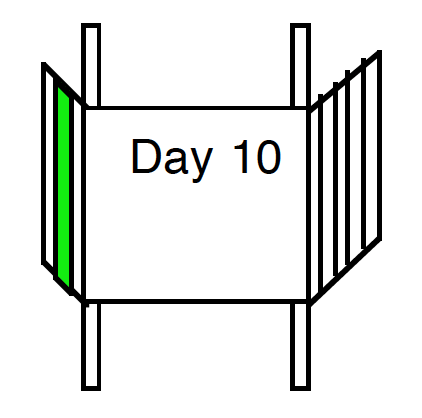
\includegraphics[height=1.4in]{fig/fig5.png}
\caption{Diagrammatic illustration of the `distortion' associated with the metaphor of the Bifocal Diary.}
\end{marginfigure}




%The design of the interface reported in this paper is influenced by many factors. Foremost are the clinically-based requirements needed to support effective interaction by a user. Of paramount importance in this connection is clear sight of current blood glucose data and any recommendations (e.g., of insulin dosage) that would directly impact upon blood glucose levels.  The ability to display the glycaemic impact following similarly encountered recommendations, and vice versa, provides context and instils confidence in decisions recommended by the system. Other factors include preferences expressed by users, elicited via meetings at which possible interface designs are critiqued, as well as the limited display area provided by a hand-held device. Overall, in the design of an interface to address all these factors, generally agreed guidelines (e.g., \cite{Elmqvist-FluidInt2011}) concerning human-system interaction must be followed to ensure that the cognitive load imposed on a user is minimized.


\section{Interface Design}

The design of the interface reported in this paper is influenced by many factors. Foremost are the clinically-based requirements needed to support effective interaction by a user. Of paramount importance in this connection is clear sight of current blood glucose data and any recommendations (e.g., of insulin dosage) that would directly impact upon blood glucose levels.  The ability to display the glycaemic impact following similarly encountered recommendations, and vice versa, provides context and insulin confidence in decisions recommended by the system. 

%\subsection{Clinical Considerations}
Following a detailed review by specialist diabetologists of current diabetes decision support systems, five groupings of data required from, and to be presented to, the user were identified.  These were: (1)	Blood Glucose: graphical presentation of blood glucose data over the last six hours and access to continuous historical data on a displayed diary. 
%Time-stamped meal and exercise data provide context for variations in blood glucose levels.
(2)	Food: parameters such as carbohydrate (`carb') and protein values as well as alcohol intake.
(3)	Exercise: A categorical choice of planned exercise type and intensity.% (e.g. aerobic, anaerobic; light, moderate, and heavy)
(4)	Health: The ability to trigger AI adaptations during periods of stress and intercurrent illness as well as to access recorded customizable parameters significant to the management of diabetes. %These include filter-adjusted blood glucose measurements, and stress and illness, among others.
(5)	Advice: Presentation of trends associated with negative outcomes on blood glucose levels.
%The provision of both preventative advice and context via events displayed on a diary.

%\subsection{The human visual system}

%The effectiveness of user interaction with a hand-held device is crucially dependent upon the nature of the human visual system, so related potential issues associated with retinopathy and neuropathy have been addressed. 

%One such is retinopathy and neuropathy. These are common diabetes complications that can manifest as reduced visual acuity and peripheral sensory neuropathy. Another issue is associated with impaired colour vision which can also occur in individuals with and without established retinopathy \cite{Gella-Impairment2015,Tan-FactorsAss2017}. Most common cases of impaired colour vision affect the red-green axis, but cases of blue-yellow impairment (tritanopia) have been identified in diabetes populations \cite{Tan-FactorsAss2017}. To overcome neuropathy our interface will utilise the haptic vibration feedback feature within smartphone hardware. The ability to scale text; the use of customizable pictures/icons; and the avoidance of high contrast colours (red, green, blue and yellow) will all support accessibility to users having impaired colour and visual acuity.



\subsection{User Preferences}

A series of focus meetings with people with T1DM, observed by clinicians, engineers and experts in human computer interaction, supported the co-design of the app. The identification of four principal input data types (Food, Exercise, Health, Advice) was agreed within the focus meetings, with an emphasis on ensuring that important data associated with each type could remain visible as interaction proceeds. The result of interaction design is illustrated in Figures 1 to 6 and summarized below.


%Variety in meal choices are often limited within the constraints of stable dietary intake behaviour determined by multiple factors including eating habits and core food environment. This stable behaviour results in choices within a set food category with minimal impact on core dietary patterns \cite{mela-Food1999}. The inclusion of features that allow the patient to save and choose previously entered meal profiles via the display of meal images can exploit habitual dietary behaviour and make the process of meal selection easy and efficient. 


%Our aim was to co-design the ARISES app with potential future users. Indeed, a multidisciplinary design mode engaging potential users throughout the design process is a recommended strategy for improving mobile health applications \cite{Ben-Priciples2015}. Co-designing the ARISES app alongside individuals with T1DM ensured their opinions were understood and appropriately represented. To this end a series of semi-structured focus meetings with people with T1DM, and observed by clinicians, engineers and experts in human computer interaction, provided a forum to gather feedback regarding data representation and presentation. Questionnaires and outcomes documented in real-time during each meeting were distributed among participants for validation.

%T1DM participants strongly recommended that, to avoid therapeutic errors, current blood glucose levels, insulin dose recommendations and insulin-on-board (insulin still active in the body from previous doses) are clearly and unambiguously presented within the interface. Most continuous blood glucose sensor applications will alert patients when the level falls outside a target range, but the majority of patients can anticipate, and are sensitive to, physiological symptoms that occur when blood glucose levels deviate to extremes. The ability to modify alert thresholds for blood glucose, and provide advisory support, were vital functions suggested to avoid user fatigue.

%The identification of four principal input data types (Food, Exercise, Health and Advice) was agreed within the focus meetings, with an emphasis on ensuring that important data associated with each type could remain visible as interaction proceeds.

%Focus groups also confirmed and extended our understanding of habitual behaviour to meal choices and physical activity. Variety in meal choices are often limited within the constraints of stable dietary intake behaviour determined by multiple factors including eating habits and core food environment. This stable behaviour results in choices within a set food category with minimal impact on core dietary patterns \cite{mela-Food1999}. The inclusion of features that allow the patient to save and choose previously entered meal profiles via the display of meal images can exploit habitual dietary behaviour and make the process of meal selection easy and efficient. The same concept is transferable to the input of exercise choices.

%The ability to review the glycaemic outcomes of historic events was considered to be an important feature in the support of future treatment decisions. For example, the incorporation of a customizable event and data filter in the Health region, and using a diary to visually review the circumstances surrounding blood glucose outcomes, delivers an ingeneous level of precision and context in presenting historical data. Such a feature not only indicates when specific events and outcomes occur but helps to explain why and what factors could have contributed. A general statistics pop-up accessible in the Health domain will provide users with a welcome snapshot of daily, weekly or monthly data (e.g., daily insulin requirements, percentage time in glycaemic range, frequency of hypoglycaemia and exercise data).  The impact of intercurrent illness and stress on blood glucose levels is well documented in the medical literature \cite{Lloyd-Stress2005}. The addition of a stress and illness switch was suggested to alert the artificial intelligence to make algorithm adaptations. A clearly visible icon on the diary will serve as a reminder to the user to switch this feature off following recovery.

%\subsection{Design decisions}

%All the above considerations led to five principal design decisions, described below in section 4. They concern data menu structure (section 4.1), context visibility (section 4.2), temporal presentation (section 4.3), challenges imposed by limited display area (section 4.4) and the benefit of so-called dynamic exploration (section 4.5). Together, these design decisions led to a novel hand-held interface anticipated to be supportive of a person's self-management of Type-1 diabetes..


%\section{The Interface}
%The overall layout of the new interface is shown in Figure 1.  The upper part provides an interactive diary allowing temporal data to be presented, and easily explored, both qualitatively and quantitatively. The lower part permits the input and viewing of data regarding Food, Exercise, Health and Advice.

%\subsection{Data Regions}

%\begin{marginfigure}
%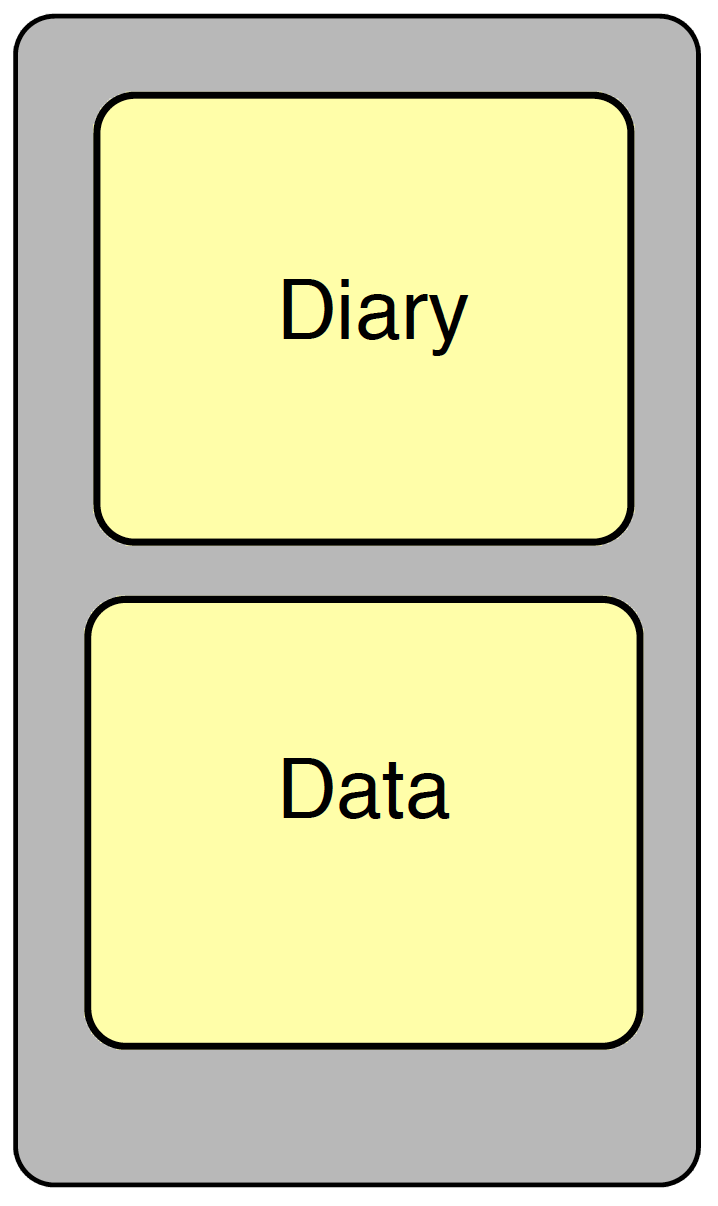
\includegraphics[height=4in]{fig/fig1.png}
%\caption{The allocation of display area to temporal data (top) and data input and output (lower). }
%\end{marginfigure}


%\begin{figure}
%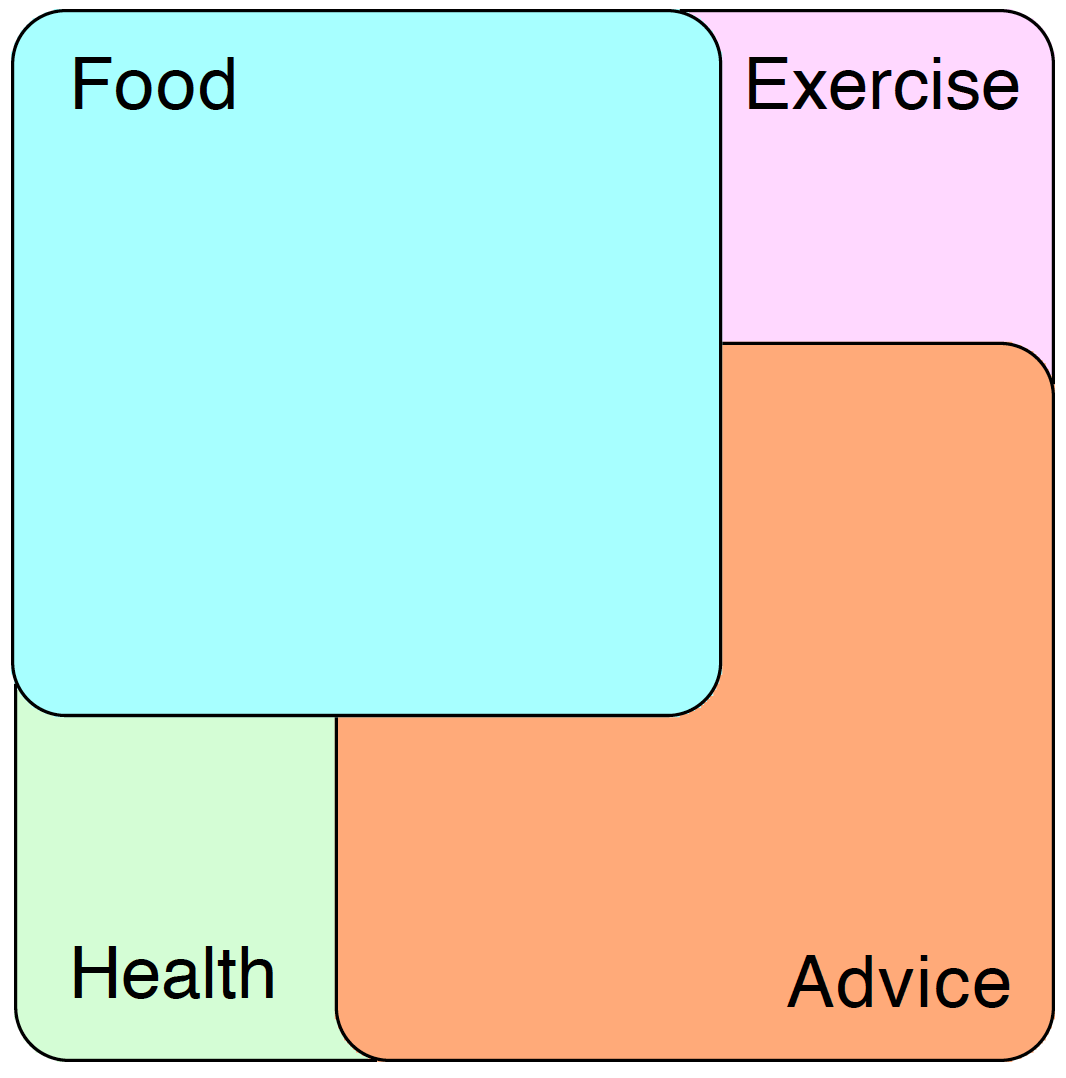
\includegraphics[height=2.5in]{fig/fig2.png}
%\caption{Layout of the four data regions occupying the lower part of the hand-held display.}
%\end{figure}



%\begin{figure}
%\centering
%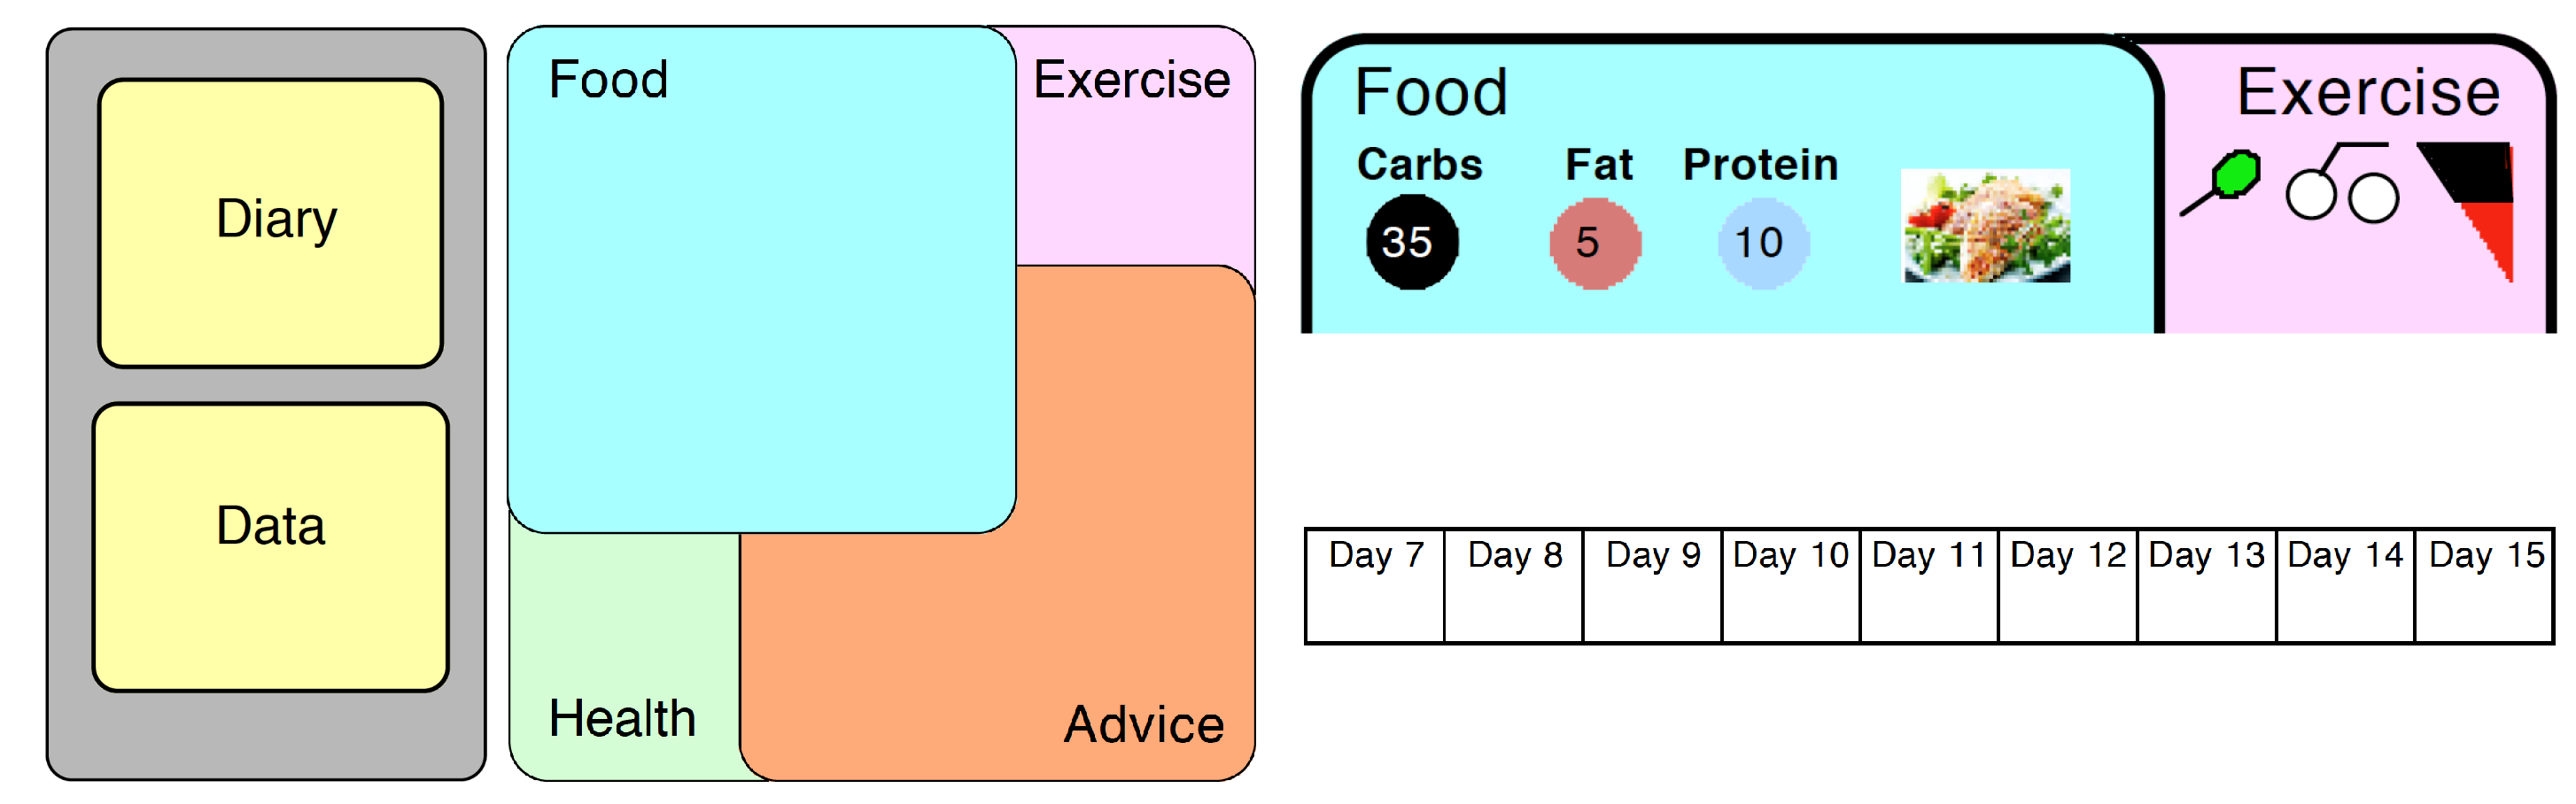
\includegraphics[height=1.5in]{fig/fig1_4.png}
%%\caption{Left: The allocation of display area to temporal data (top) and data input and output (lower). Right: Layout of the four data regions occupying the lower part of the hand-held display.}
%\caption{left: Fig. 1.1; middle: Fig. 1.2; right upper: Fig.1.3; right lower: Fig.1.4.}
%\end{figure}
%%\vspace{-0.3\baselineskip}



%Fig. 1: shows the allocation of display real estate to temporal data (upper) and fixed data (lower). Fig. 2: overlapping regions are associated with important variables. Touch on any region brings it to the top of the stack, leaving remainder in the previous order. A fixed sub-area of each region is always visible, providing valuable context. Fig. 3 is an example interactive icons allowing input of Food and Exercise data. Fig. 1.4 shows unsuitable diary presentation. 

Fig. 1 (left) shows the allocation of display real estate to temporal (upper) and fixed (lower) data. Fig. 1 (right) shows overlapping regions associated with important fixed variables. Touch on any region brings it to the `top' of the stack, leaving the remainder in their previous order. A fixed sub-area of each region is always visible, providing valuable context. Fig. 2 provides an example of interactive icons allowing Food and Exercise data to be entered.  Fig. 3 shows an unsuitable diary presentation.

%The data area of the proposed interface occupies the lower part of the hand-held device and is illustrated diagrammatically in Figure 2.  A first major design decision was to place, within the data area, four overlapping rectangular regions, one for each data type. Within each region a user can make and view choices. For example, (see Figure 3) the user might select a meal from a set of images, enter the carb value of a planned snack, and choose a planned schedule of exercise for the next hour or two.

%Simple selection (touch, for example) will bring a region to `the top', leaving the other regions ordered as before. An anticipated advantage of the overlapping regions depicted in Figure 2 is the simple mental model it can provide for the user. Another feature of the proposed use of overlapping data regions is the absence of a `home state' with its often inevitable hint of hierarchy and navigational difficulties. A user seeking the concept of a `home state' will soon realize that it is the last arrangement of the data regions, a sort of `nomadic home state'. But a major consideration in the design of the overlapping regions was to ensure that a part of each region would always be visible, whichever other region is uppermost, as illustrated in Figure 3. This feature served to allow future events to be entered without losing the visual context of important data and to provide a constant visual reminder of recently entered events (past or future) that directly impact blood glucose (for example, 24-hour macronutrients and planned exercise).



%\subsection{Context visibility}

%A second design decision acknowledged the importance of context visibility.  In the example of the data regions, such context visibility was easy to achieve: whichever region is currently `uppermost', substantial portions of the other three regions are always visible, acting as an often needed reminder of an earlier choice. Those constantly visible `mini regions' are not simply the tabs conventionally supportive of navigation but extremely useful reminders of earlier major decisions.

%The value of context visibility is also supportive of three other design decisions: the choice of a mechanism for temporal data presentation (a diary) discussed in section 4.3; a mechanism for easing the entry and interrogation of data in section 4.4; and, in section 4.5, the dynamic manual exploration of the effect of one type of data on another (e.g., carbs, blood glucose and insulin dosage).



%\subsection{Temporal Data}

%\begin{figure}
%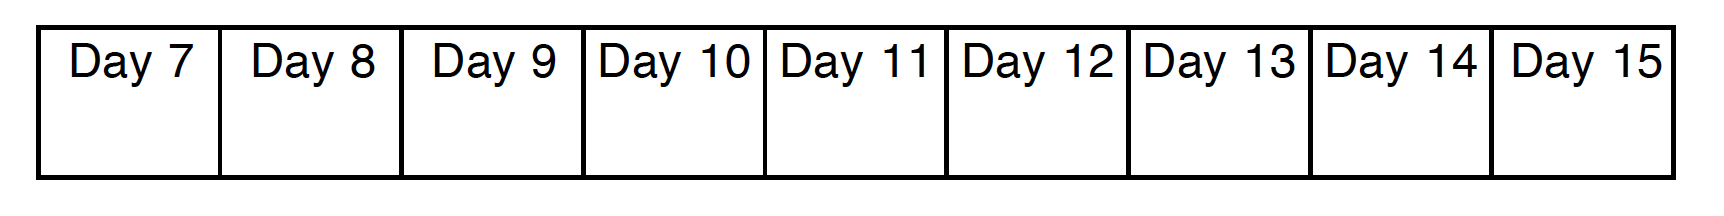
\includegraphics[height=0.4in]{fig/fig4.png}
%\caption{A linear presentation of consecutive days, having a shape unsuited to a limited display %area}
%\end{figure}

%Temporal data is key to the successful management of Type-1 diabetes: it includes the choices (e.g., of food and exercise) made over past hours and days, as well as automatically captured physiological data such as blood glucose and insulin dose. To reflect the importance of temporal data the upper part of the interface (see Figure 1) is dedicated to a diary within which that data can be viewed and interacted with.

%A conventional diary typically employs a tabular format, but that is unsuited to the small display area available, especially when two different encodings are required: one is a detailed and primarily quantitative view associated with a single day (e.g., blood glucose levels), while the other is a qualitative overview identifying features of possible interest occurring on previous days and, often, worthy of detailed study.

%\begin{figure}
%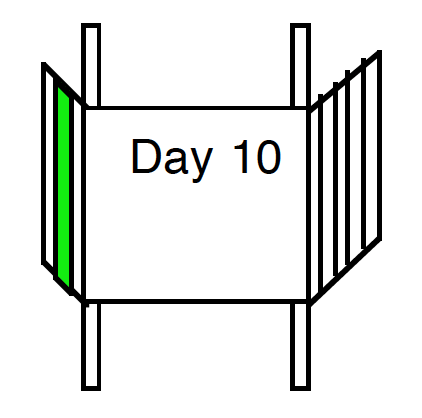
\includegraphics[height=1.7in]{fig/fig5.png}
%\caption{Diagrammatic illustration of the `distortion' associated with the metaphor of the Bifocal Diary.}
%\end{figure}

%The diary format chosen is based on a linear presentation of consecutive days (Figure 4). That shape, of course, is unsuited to a limited display area so it is `distorted', as illustrated by the metaphor termed the Bifocal Display \cite{Spence-DataBaseNav1982} as shown in Figure 5. This third major design decision permits the provision of both a quantitative view within a single day and, simultaneously, a qualitative overview of each of many days. Thus an event of interest occurring in Day 8 (for example a meal identical to the currently selected one) can be identified qualitatively at a glance (see the green colour encoding Day 8 in Figure 5) and, if judged of interest, can be brought, by scrolling, to `the front' to permit quantitative inspection.



\begin{marginfigure}
\centering
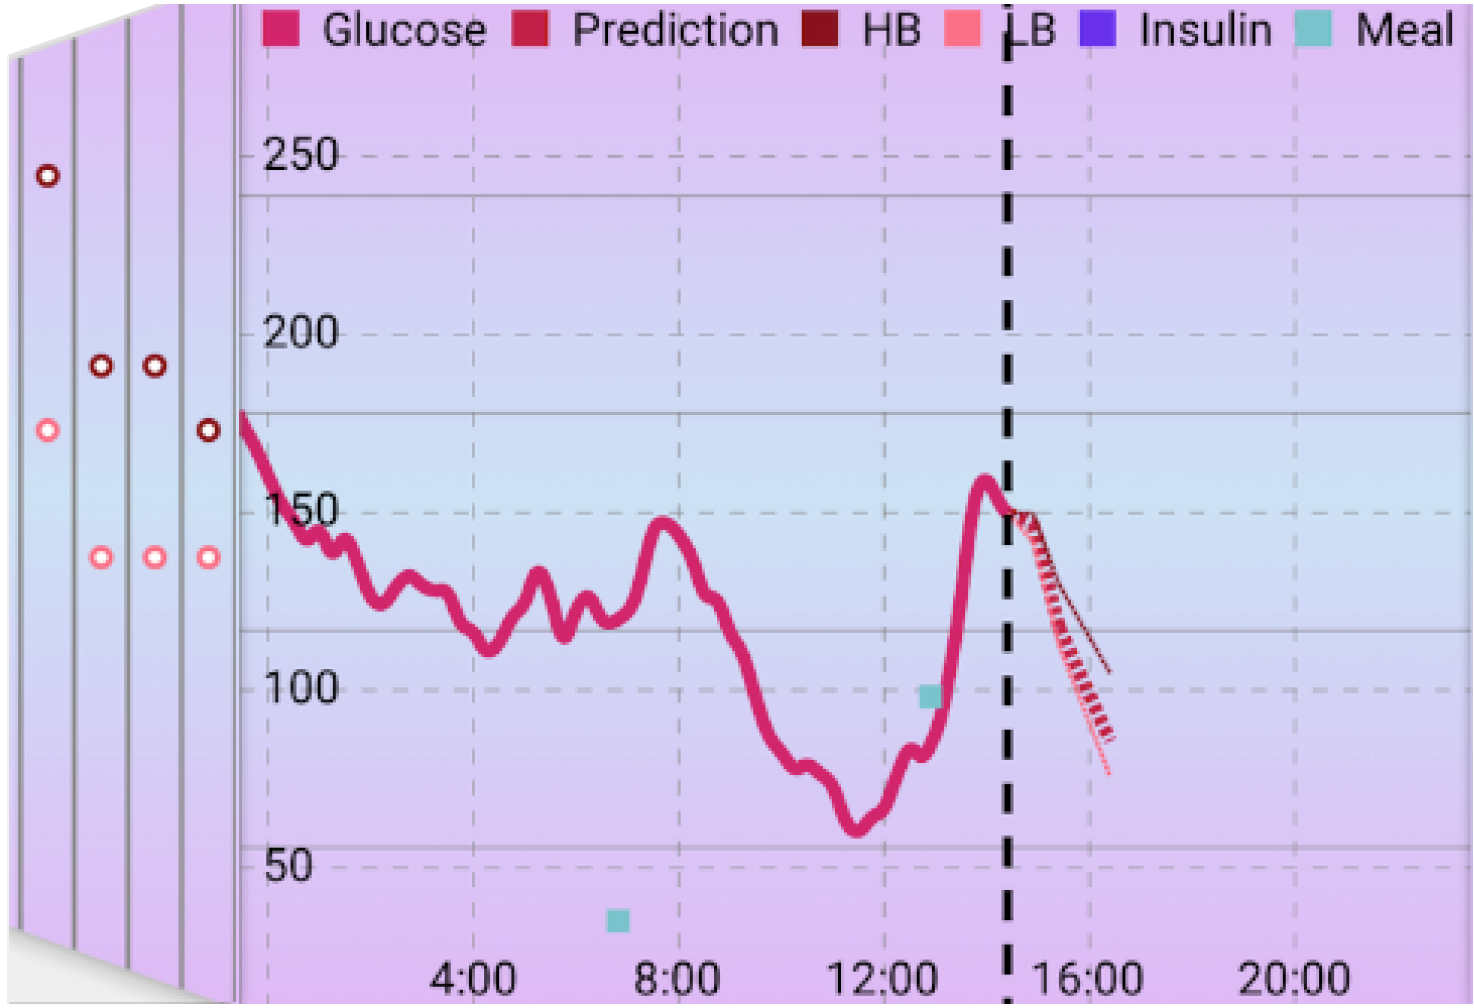
\includegraphics[height=1.3in]{fig/fig6.png}
\caption{The actual (before the vertical black line denoting `Now`) and predicted variation of blood glucose for the current day.}
\end{marginfigure}



%\begin{marginfigure}
%\begin{minipage}[b]{0.99\linewidth}
%\centering
%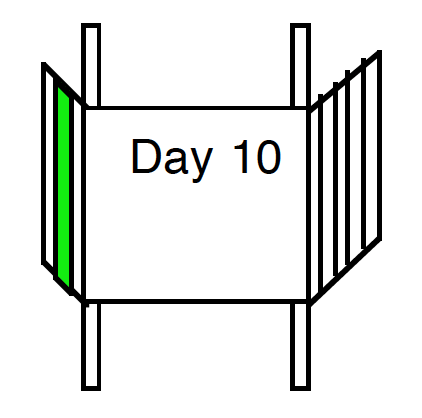
\includegraphics[height=1.8in]{fig/fig5.png}
%%\caption{The allocation of display area to temporal data (top) and data input and output (lower). }
%\end{minipage}% <- this is important here
%\begin{minipage}[b]{0.99\linewidth}
%\centering
%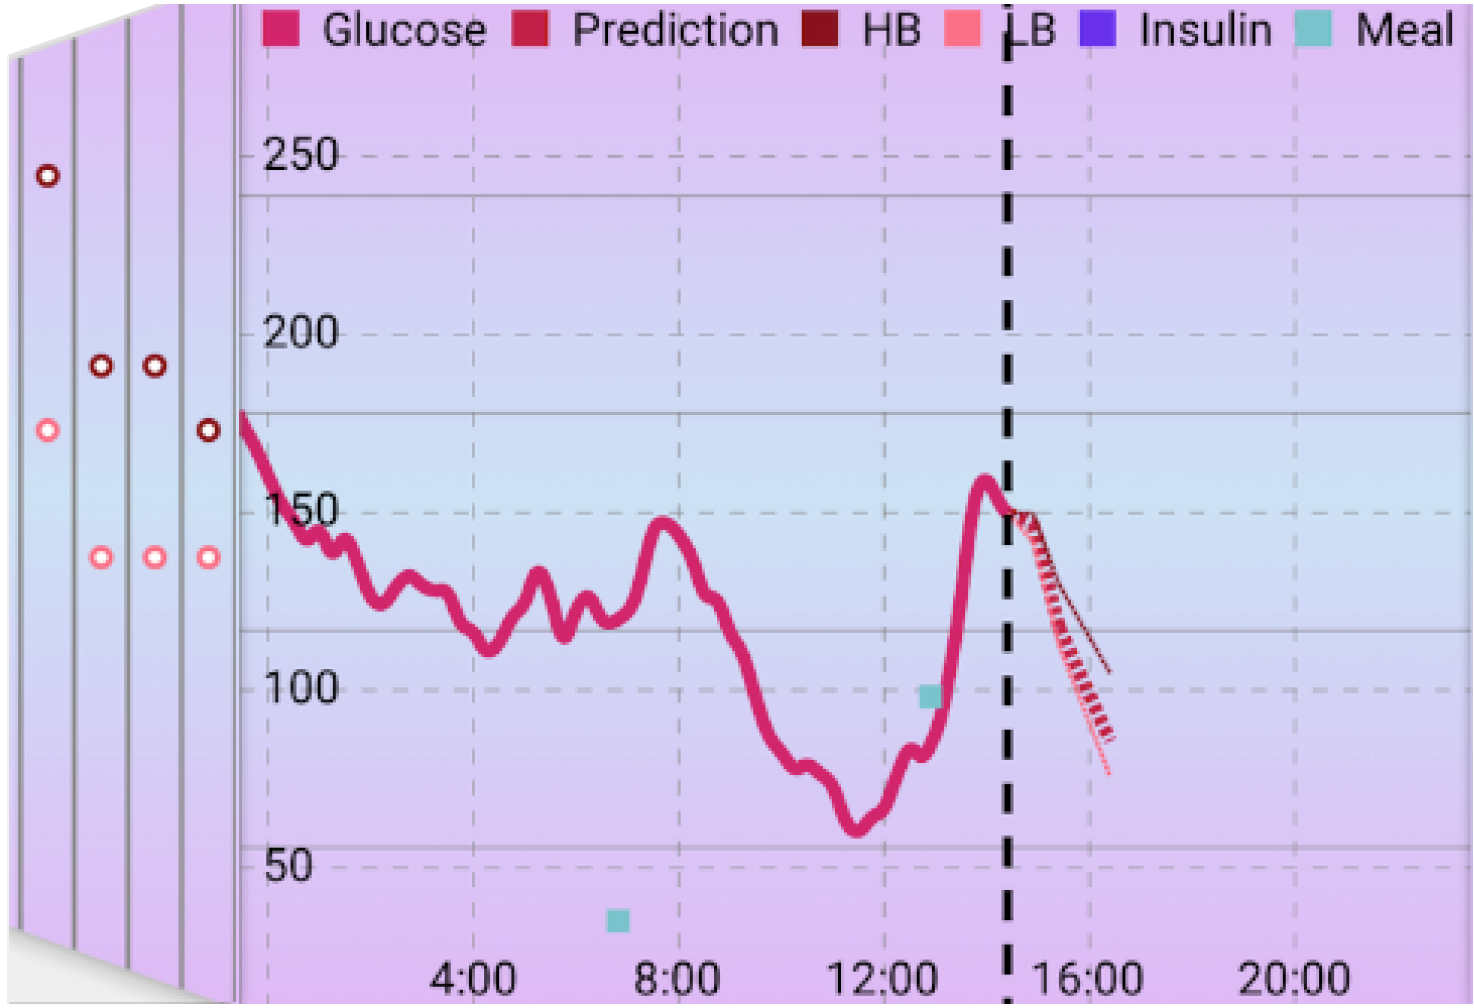
\includegraphics[height=1.5in]{fig/fig6.png}
%\caption{Layout of the four data regions occupying the lower part of the hand-held display.}
%\end{minipage}
%\caption{Left: Diagrammatic illustration of the `distortion' associated with the metaphor of the Bifocal Diary. Right: The actual (before the vertical black line denoting `Now`) and predicted variation of blood glucose for the current day.}
%\caption{Left: distortion of diary to provide a diary showing quantitative detail for a single day and summary qualitative detail for adjacent days. Right: An example for the current day showing, in the focus region, the detected and predicted blood glucose level: dashed vertical line indicates `now'}
%\end{marginfigure}

%\begin{figure}
%\centering
%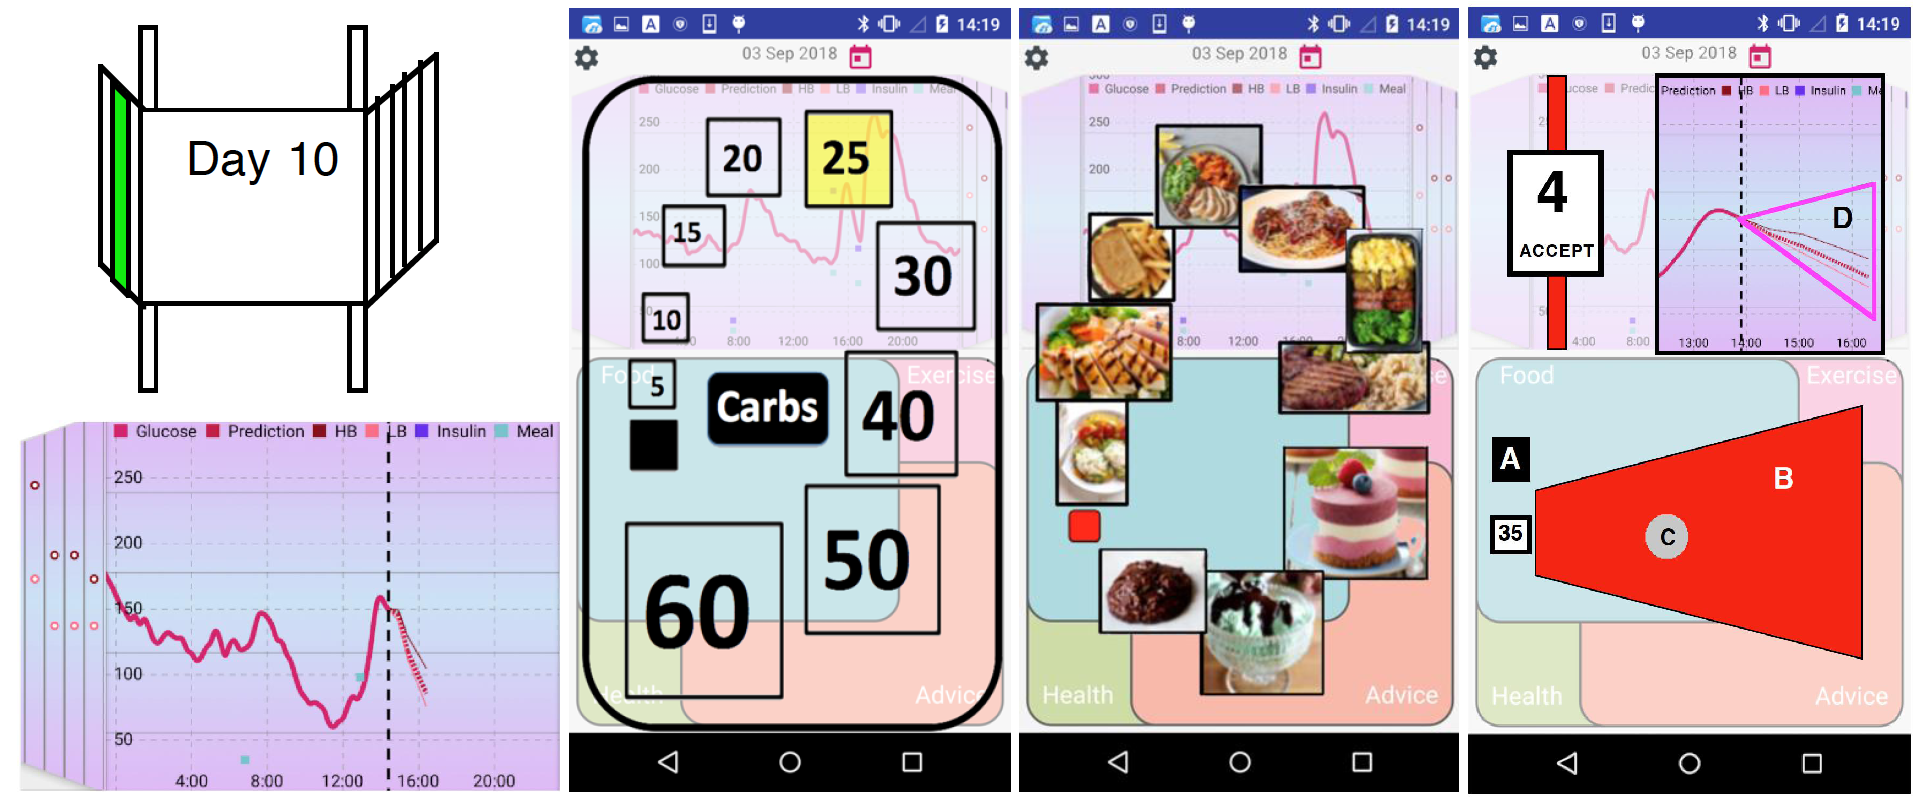
\includegraphics[height=2.3in]{fig/fig5_7.png}
%\caption{left upper: Fig.2.1; left lower: Fig.2.2; mid left: Fig.2.3; mid right: Fig.2.4; right: 2.5.}
%\end{figure}
%\vspace{-0.3\baselineskip}

Fig. 4 shows how distortion of the unsuitable presentation of Fig. 3 can provide a diary showing quantitative detail for a single day and summary qualitative detail for adjacent days. Fig. 5 is an example for the current day showing, in the focus region, the detected and predicted blood glucose level: dashed vertical line indicates `now'. Fig. 6 (left) shows that when entering carbohydrate levels, a user need only pay attention to available values, so the remainder of the display is rendered inconspicuous, though present to provide context. People are creatures of habit, so the ARISES app provides, on request (Fig. 6 centre) a slowly moving carousel of past meals, allowing easy selection.  The interface also allows (Fig. 6 right) a user to ask (in this example) the question ``What will happen to my blood glucose level if I (a) select different carb values by a finger slide along the (red) carb range, or (b) explore different insulin doses ?'' Both (a) and (b) result in the immediate display of results, calculated by a machine-learning algorithm.



%Fig.4 shows the distortion of days to provide a diary showing quantitative detail for a single day and summary qualitative detail for adjacent days. Fig. 5 is a example for the current day showing, in the focus region, the detected and predicted blood glucose level: dashed vertical line indicates `now'. Fig. 6 Left shows when entering carbohydrate levels, a user need only pay attention to available values, so the remainder of the display is rendered inconspicuous, though present to provide context. People are creatures of habit. The ARISES app provides, on request, a slowly moving carousel of past meals, allowing easy selection, as shown in Fig. 6 Mid. In Fig. 6 Right, the interface allows a user to ask (in this example) ``What will happen to my blood glucose level if I (1) select different carb values (by finger slide along the red carb range), or (2) explore different insulin levels?'' Both (1) and (2) result in immediately displayed results, calculated by a machine-learning algorithm.

% 6 shows, in the central (`focus') area of the Bifocal Diary, a view of a typical current day. The red line shows the patient's blood glucose (BG) level as measured automatically at 5 minute intervals up to the current time, and then as a predicted continuous curve with associated confidence levels for the next two hours.  The prediction is based on historical data \cite{Li-ConvRecNN2018}. Also shown in the `today' area are events such as past insulin dose recommendations.

%In the `distorted' area to the left of the `today' area in Figure 6, qualitative indications of blood glucose minima and maxima levels are displayed: events such as a meal identical to the one just chosen could be similarly encoded. If any such information is of detailed interest, a horizontal finger movement across the diary will lead to the day of interest moving and then `snapping' into the focus region, with content similar to that shown in Figure 6.


%\subsection{Area constraints}
%A considerable challenge arises from the limited area available on a typical hand-held display, especially for users with visual impairment, limited finger dexterity and tremor.  The approach taken was based on the assumption that, during the brief (e.g., 2 sec) selection of  a value or item, the user's attention need not be paid to, or distracted by, anything irrelevant to that action. This assumption has consequences for many actions, two of which are now discussed.

%A considerable challenge can arise from the limited area available on a typical hand-held display, especially for users with visual impairment, limited finger dexterity or tremor. The fourth major design decision (comprising a number of separate techniques) addressed this general but pressing problem, and was based on a simple assumption: that, during the selection of a value or item  (e.g., carbs value) the user's attention will, for a short time (e.g., 500 to 3000 milliseconds) be focused on that action alone and will not need to be directed to any other feature of the display. This assumption has ramifications for many of the activities planned by the user: two such examples are illustrated below.

%\subsubsection{Value selection}
%Touch on an appropriate icon in the Food region causes the menu shown in Figure 5 (left) to appear: it makes full use of the display, and the background is rendered inconspicuous. Following the selection of a carb value by touch, the menu disappears and the background is restored to normal.
%Consider the situation where a user wishes to enter the carb value for an intended meal. The proposed approach involves, first (Figure 7), a touch on an appropriate icon in the Food region. That causes a menu to appear, offering a range of carb values. The menu makes use of much of the available display area, a subtle highlight of one value (25) indicating the last value selected and supporting any required fleeting reminder.  At the same time other details on the display are `ghosted' since, for a very short time, attention will not be paid to anything other than the available carb values: nevertheless, to retain valuable context information, they are not removed.


%\begin{figure}
%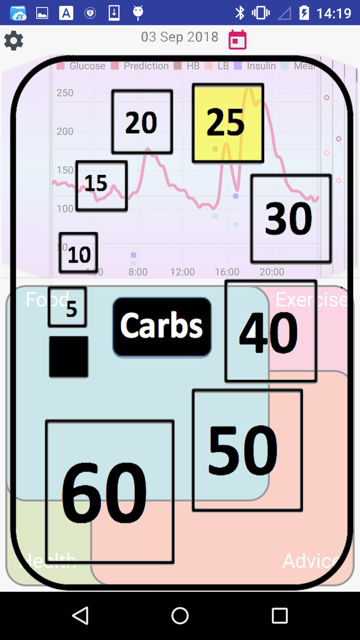
\includegraphics[height=3.1in]{fig/fig7.png}
%\caption{Menu options are more easily selected if made large. During value selection (taking, say, 500 to %2000 milliseconds), inability to see ghosted items would not be serious.}
%\end{figure}

\begin{marginfigure}
\centering
\begin{minipage}[b]{0.32\linewidth}
\centering
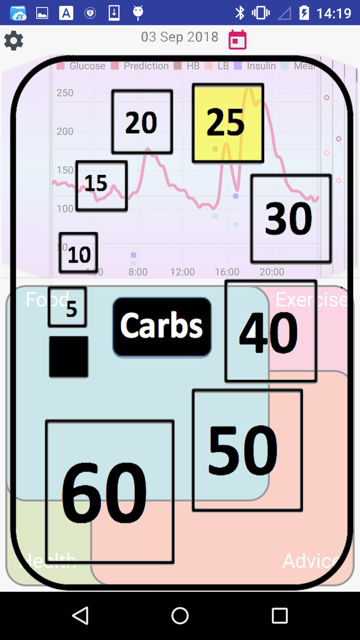
\includegraphics[height=1.25in]{fig/fig7.png}
%\caption{The allocation of display area to temporal data (top) and data input and output (lower). }
\end{minipage}% <- this is important here
\begin{minipage}[b]{0.32\linewidth}
\centering
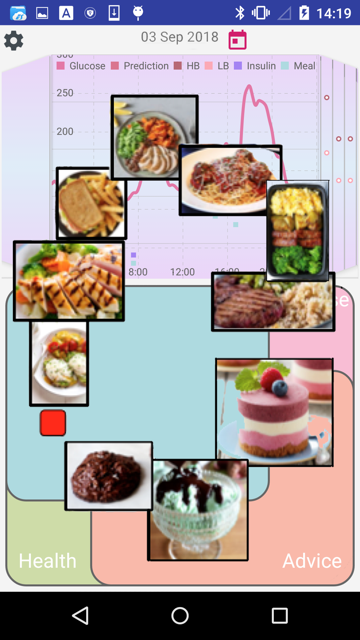
\includegraphics[height=1.25in]{fig/fig9.png}
%\caption{Layout of the four data regions occupying the lower part of the hand-held display.}
\end{minipage}
\begin{minipage}[b]{0.32\linewidth}
\centering
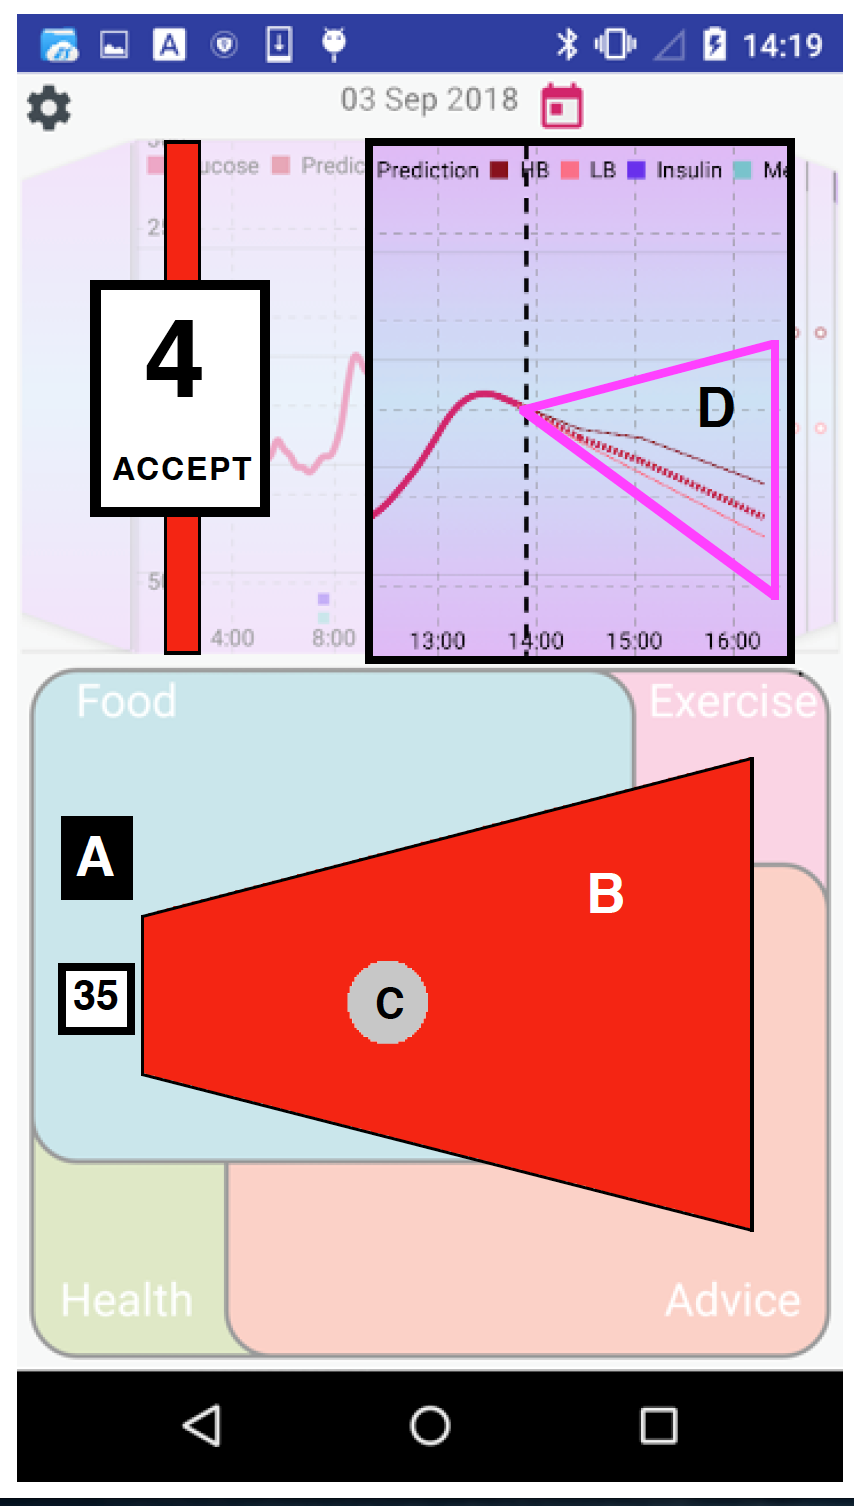
\includegraphics[height=1.25in]{fig/fig10.png}
%\caption{Layout of the four data regions occupying the lower part of the hand-held display.}
\end{minipage}
\caption{Left: Menu options are more easily selected if made large. 
%During value selection (taking, say, 500 to 2000 milliseconds), inability to see ghosted items would not be serious. 
Middle: A carousel presentation of past meals. Right: Interface appearance following touch on the icon A. \\
%A sliding touch on B and observance of the area within D supports dynamic exploration of the influence of carb value on predicted blood glucose and recommended insulin dosage.
}
\end{marginfigure}



%Next, a touch on a desired carb value causes the menu to disappear, the selected value to be entered within the icon originally touched, and the background restored to its previous state.   If an intermediate value is required, the second touch will be applied between two values, whereupon a new menu (Figure 8) offering more precision will appear.

%\begin{figure}
%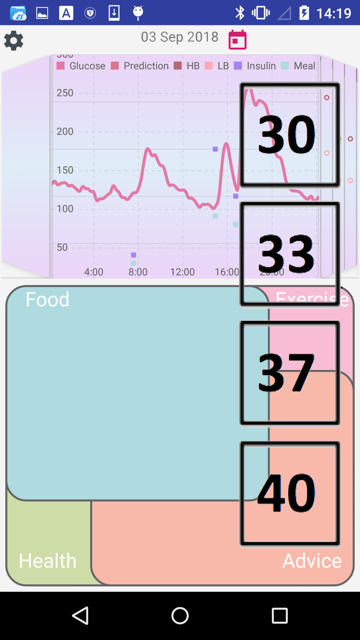
\includegraphics[height=4.6in]{fig/fig8.png}
%\caption{A menu supporting the selection of intermediate carb values }
%\end{figure}

%\subsubsection{Meal selection}

%The fact that people often choose to eat a familiar dish suggested the presentation shown in Figure 5(right) in which a slowly moving carousel \cite{Spence-ImagePre2002} of meal images allows a meal of interest to be identified and selected by touch.

%People with T1DM will often wish (see Section 3.3) to select a familiar meal consumed at an earlier date.  The same assumption underlying the supported input of carb values (section 4.4.1, Figure 7) was adopted and its application to meal selection explored. Following a touch on an appropriate icon in the Food Region, a slowly moving carousel \cite{Spence-ImagePre2002} of meal images emerges from, and eventually returns to, that icon: its trajectory occupies much of the display area (Figure 9) and its speed of movement is sufficiently slow to permit easy selection of an image by touch. Following meal selection, the carousel disappears.

%\begin{figure}
%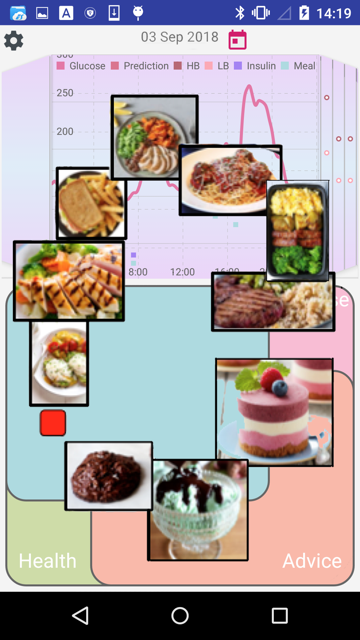
\includegraphics[height=3.2in]{fig/fig9.png}
%\caption{A carousel presentation of past meals. }
%\end{figure}



%\subsection{Dynamic Exploration}

%User trepidation surrounding the self-management of T1DM stems largely from uncertainty about how blood glucose levels will change in response to daily choices such as meals, exercise and recommended insulin dosage. What the user would like to do is ask a ``what if?'' question such as ``If I increased the carb value of the meal I am just about to eat, how will that affect my predicted blood glucose over the next two hours and the recommended insulin dosage? And if I then varied the recommended insulin dosage what would happen to my blood glucose for the same meal?''

%To enable such exploration, continuous glucose monitoring records blood glucose levels every five minutes. Advanced machine learning algorithms then enable the ARISES app to make a prediction of blood glucose levels over the next two hours for a variety of hypothetical scenarios. That prediction can be essentially immediate, enabling the user to continuously vary a carb value and immediately see its effect, a process known as dynamic exploration \cite{Spence-InfoVis2014,Neufeld-ExtendingTheDim2008}.

%\begin{figure}
%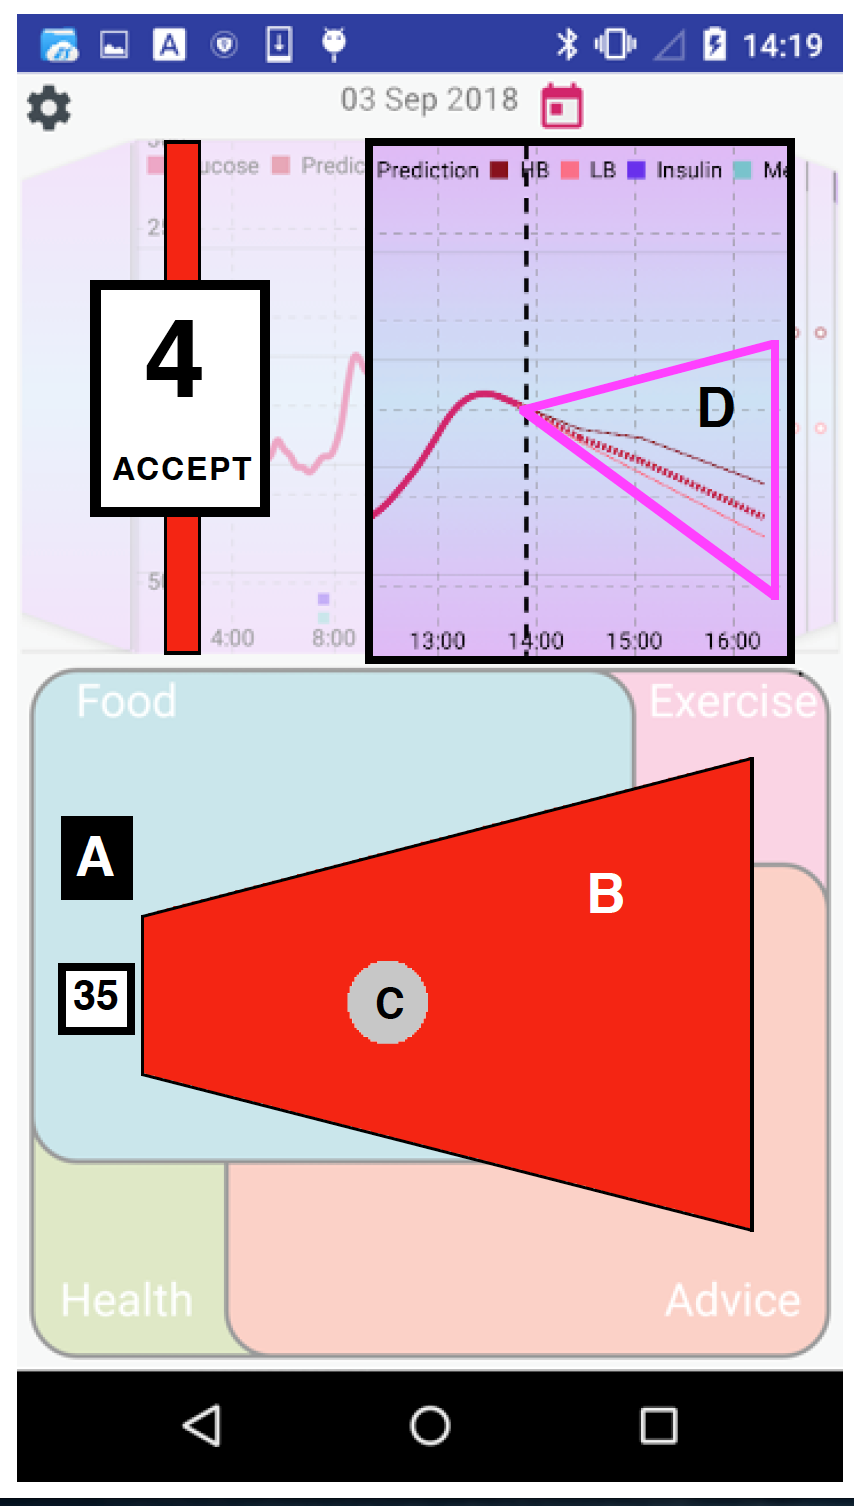
\includegraphics[height=2.7in]{fig/fig10.png}
%\caption{Interface appearance following touch on the icon A. A sliding touch on B and observance of the area within D supports dynamic exploration of the influence of carb value on predicted blood glucose and recommended insulin dosage.}
%\end{figure}

%A proposed interface to support dynamic exploration of the effect of carb value on predicted blood glucose and insulin dose is shown in Figure 10. Briefly, a touch on A causes the appearance of the red area B which is a `carb slider' with high values at the right and a current value indicated by C. The frame D shows the predicted blood glucose for the next two hours and its possible limits, while the recommended bolus value of insulin is shown by the integer (here 4) in a box.  Importantly, the background is rendered inconspicuous. Sliding a finger  horizontally along the carb slider B causes an immediate change in the predicted glucose level and bolus value.


%User trepidation surrounding the self-management of T1DM stems largely from uncertainty about how blood glucose levels will change in response to daily choices such as meals, exercise and recommended insulin dosage. What the user would like to do is ask a ``what if?'' question such as ``If I increased the carb value of the meal I'm just about to eat, how will that affect my predicted blood glucose over the next two hours and the recommended insulin dosage? And if I then varied the recommended insulin dosage what would happen to my blood glucose for the same meal?''

%To enable such exploration, continuous glucose monitoring records blood glucose levels every five minutes. Advanced machine learning algorithms then enable the ARISES app to make a prediction of blood glucose levels over the next two hours for a variety of hypothetical scenarios. That prediction can be essentially immediate, enabling the user to continuously vary a carb value and immediately see its effect, a process known as dynamic exploration \cite{Spence-InfoVis2014,Neufeld-ExtendingTheDim2008}.  It would additionally be beneficial if the recommended insulin dosage can also be varied by manual sliding of the insulin box, and lead, for a given carb value, to a predicted blood glucose variation.

%A proposed interaction mechanism to support dynamic exploration of the effect of carb value on predicted blood glucose and insulin dose is shown in Figure 10. There are three affordances: the small icon A, the carb slider B and the insulin slider  (shown at a bolus value of 4). A touch on icon A causes, simultaneously: (1) the appearance of slider B (shaped to suggest a range of carb values); (2) an indication of a recommended insulin dose (here, a value of 4); (3) within B, and by means of a small circle (C) also suggesting touch, an indication of the carb value corresponding to the prediction of blood glucose in the bifocal diary; (4) the ghosting of all parts of the interface except for A, B, a relevant area within the bifocal diary and the recommended insulin dose; (5) by means of red boundaries (D) above and below the predicted variation of blood glucose, the range corresponding to the available range of carb value (B) (to give some idea of sensitivity), and (6), a gentle animation within B (simulating finger movement) and the corresponding animation of the prediction of blood glucose and recommended insulin dosage.

%The user can now choose from two actions. A second touch on icon A will cancel all the above activity and return the interface to its previous state. Alternatively, the action of sliding a finger along the area B (to simulate carb value change) will immediately cause the corresponding change in predicted blood glucose and recommended insulin dose to be shown in the bifocal diary.  Lifting the finger off area B then automatically selects the corresponding carb value and, within a short delay  (or by touching icon A again), the interface reverts to its previous state. There is no need for precision in the finger sliding on B. In the same way, a finger induced vertical movement of the box containing the recommended insulin dose will, for the chosen carb value, be brushed into a corresponding prediction of blood glucose.

%Dynamic exploration is capable of generalization to any parameter that influences blood glucose or any other dependent variable. It could, for example, support exploration of the interaction between caffeine (in the Food region) and potential warnings about hypoglycaemia (in the Advice region).



%\subsection{User consultation}

%As the interface design evolved, it was presented to focus groups for comment. A hierarchy-free design and the separation of input domains from output data such as blood glucose outcomes and therapeutic recommendations, was well received by users.  Similarly, the ability to dynamically explore in real-time how combinations of various input parameters affected output data (e.g., predicted blood glucose) was unanimously accepted as a positive addition.

%\section{Interaction Dynamics}
%The interface's usability is of prime consideration. There is a need not only to minimize the cognitive load imposed on the user but also to acknowledge the challenges posed by visual impairment, finger dexterity and tremor. Features already mentioned above had these priorities in mind. However, quite separately, the dynamics of interaction play an important part in the usability of an interactive system.

%Under the generic title of Fluid Interaction, Elmqvist et al \cite{Elmqvist-FluidInt2011} have drawn attention to interaction guidelines which, if followed, can substantially enhance the usability of an interface, mainly by minimizing the cognitive load experienced by a user. Their detailed practical recommendations leading to effective; indeed, rewarding - interaction experiences have been followed: major ones are discussed briefly below.


%\subsection{Fluid rather than Instantaneous change}

%The effect of interactively induced change is typically displayed instantaneously.  However, such behaviour can be disadvantageous for two reasons. One arises from that feature of the human visual system known as Change Blindness \cite{Rensink-ToSeeOrNot1997}. Another \cite{Robertson-ConeTrees1991} is due to the well-established fact that, if an instantaneous visual change occurs, considerable cognitive effort may be needed to update the user's mental model of the system. For these two reasons the implementation of our interface ensures that the effect of any interaction/touch is animated smoothly over a period of around 200 to 500 milliseconds.

%\subsection{Conceptual model}
%An interactive interface should reinforce a clear conceptual model. In other words the user should always have a clear idea of the state of the system, operations should be reversible, and connections between views should be clear and visible. This guidance has been followed in the design of our interface. One example in the data domain is the anticipated simple mental model of the overlapping regions and their ordering during interaction.


%\subsection{Dead ends}

%The user should never reach a `dead end' from which they can no longer proceed. The evaluation stage will check to see if our design satisfies this requirement.

%\section{Prototype evaluation}

%Formal user interface validation studies will be performed before and during clinical trials assessing the technical proof of concept and the efficacy of the ARISES app. Hand-device interaction will be video recorded while participants are assessed performing a series of tasks in one-to-one sessions. Software within the interface will log participant interactions and measure outcomes such as number of clicks and time taken to complete tasks.

%\section{Discussion}

%The new interface design will continue to be explored and developed and then implemented to realize a prototype that can support a usability study.

%The various techniques brought together in the proposed new interface must be implemented and then subjected to usability studies in order to assess their benefits and drawbacks. At the same time there is a need to explore many different variants of the examples provided with regard to representation, presentation and interaction. Related design decisions. For example, whether a data region could temporally be expanded to provide more space for data input, are delayed pending the outcome of user trials and discussions with users.

%Many variations of the scheme described above are possible and will be explored during the evaluation stage. Within meal choice (section 4.4.2), for example, the user could be enabled to create meal images with a camera facility. Another variation is to adjust meal image size according to some significant (e.g., carb) value. Yet another is to incorporate numerical carb values within the meal images.

\section{Conclusion}
%A novel hand-held interface has been developed to support people with Type-1 diabetes.

A hand-held interface has been developed to support people with Type-1 diabetes in the management of their condition. It combines a number of novel approaches to deliver a usable interface which will maximise its adoption by patients, impacting on chronic disease management.
%It is novel in that it brings together five approaches to meet the challenges that arise from such as application. 
%As with any other new interface its benefits and drawbacks will only be identified via usability studies employing participants with type 1 diabetes.

%in the management of their condition, and will shortly be assessed for usability.

\begin{sidebar}
\textbf{ACKNOWLEDGMENTS}\\
We gratefully acknowledge the contributions of Camille Demasson, Rebecca Elkington, Jack Pearson, Dan Wells, Ryan Armiger and Xiaoyu Ma as well as useful consultations with Taiyu Zhu. The work was supported by EPSRC EP/P00993X/1. K. Li is the corresponding author. 
\end{sidebar}

%\bibliographystyle{ACM-Reference-Format}
\bibliographystyle{abbrv}
\bibliography{sample-base}

\end{document}
